\documentclass{article}
% Text %
%%%%%%%%
\usepackage[utf8]{inputenc}
\usepackage[spanish]{babel}
\usepackage{enumitem}
% Images %
%%%%%%%%%%
\usepackage{graphicx}
\graphicspath{ {./images/} }
% Math packages %
%%%%%%%%%%%%%%%%%
\usepackage{amsmath}
\usepackage{amsthm}
\usepackage{amsfonts}
\usepackage{amssymb}
\usepackage{physics}
\usepackage{bbm}
% Math symbols %
%%%%%%%%%%%%%%%%
\DeclareMathOperator{\prob}{\mathbb{P}}
\DeclareMathOperator{\Exp}{\mathbb{E}}
\DeclareMathOperator{\Exponential}{\text{Exp}}
\DeclareMathOperator*{\argmin}{\text{argmín}}
\newcommand{\symmetric}{\mathbb{S}}
\newcommand{\naturalnum}{\mathbb{N}}
\newcommand{\realnum}{\mathbb{R}}
\newcommand{\characteristic}{\mathbbm{1}}
\newcommand{\almostSurely}{\text{ctp}}
% Math environments %
%%%%%%%%%%%%%%%%%%%%%
\newtheorem{theorem}{Teorema}
\newtheorem{lemma}{Lema}
\theoremstyle{definition}
\newtheorem{definition}{Definición}
\newtheorem{exercise}{Ejercicio}

\title{Ejercicios para entregar}
\author{Pablo Brianese}

\begin{document}
\maketitle

\begingroup
% Group variables %
%%%%%%%%%%%%%%%%%%%
\newcommand{\queueProcess}{(X_t)_{t \geq 0}}

\begin{exercise}
Consideremos un sistema que tiene un único servidor, que atiende a tasa $\mu > 0$, y los clientes llegan a tasa $\lambda > 0$.
Sea $X_t$ la cantidad de clientes que hay en la cola a tiempo $t$, con $t \geq 0$.
Notar que $\queueProcess$ es un proceso de Markov a tiempo continuo.
(Este modelo, llamado $M/ M / 1$, lo hemos charlado en la clase práctica 20 y 23).
\begin{enumerate}[label=\alph*)]
    \item Probar que el proceso es recurrente positivo si y sólo si $\lambda < \mu$.
	Con lo cual, empezando con la cola vacía, el tiempo medio que tarda la cola en volver a vaciarse es finito si y sólo si $\lambda < \mu$.
	\item Asumiendo $\lambda < \mu$, calcular la proporción (asintótica) de tiempo que la cola está vacía.
\end{enumerate}
\end{exercise}

\begin{proof} a)
Comezamos analizando este proceso como lo hicimos en la clase práctica número 20.

% Cálculo de la matriz generadora del proceso %
%%%%%%%%%%%%%%%%%%%%%%%%%%%%%%%%%%%%%%%%%%%%%%%
% Nota 25 nov. 2020 teoría de proba  clase práctica 20.pdf %
%%%%%%%%%%%%%%%%%%%%%%%%%%%%%%%%%%%%%%%%%%%%%%%%%%%%%%%%%%%%
% Vamos a ver que \(\Exp(T_0) < \infty\) si y solo si \(\lambda < \mu\).

% Si la cadena está en el estado 0, sólo puede saltar al 1; si está en un estado \(i > 0\), puede saltar a \(i - 1\) o a \(i + 1\).

% Si está en 0, salta al estado 1 cuando suena un reloj exponencial de parámetro \(\lambda\).
% Si se encuntra en un estado \(i > 0\), hay dos relojes exponenciales compitiendo, uno a tasa \(\lambda\), que indica la llegada de una persona y otra a tasa \(\mu\) que indica que una se va. 

% Usaremos los siguientes lemas sobre la distribución exponencial:
% \begin{enumerate}
% 	\item Si \(X \sim \Exponential(\lambda)\), entonces \(\prob(X > t + s | X > s) = \prob(X > t)\).
% 	\item Si \(\{X_i\}_{i \in \naturalnum_0}\) son v.a. independientes con distribuciones \(X_i \sim \Exponential(\lambda_i)\) tales que \(\sum_{i \in \naturalnum_0} \lambda_i\), entonces
% 	\begin{itemize}
% 		\item \(\min_{i \in \naturalnum_0} X_i \sim \Exponential(\lambda)\) con \(\lambda = \sum_{i \in \naturalnum_0} \lambda_i\)
% 		\item \(\prob(\argmin_{i \in \naturalnum_0} X_i = j) = \lambda_j / \lambda\), con \(\lambda = \sum_{i \in \naturalnum_0} \lambda_i\), para todo \(j \in \naturalnum_0\).
% 	\end{itemize}
% \end{enumerate}

% Usando estos lemas, podemos pensar que estando la cadena en el estado \(i > 0\), su cambio responde a un único reloj exponencial con tasa \(\lambda + \mu\), y al sonar este reloj se tira una moneda cargada:
% con probabilidad \(\lambda / (\lambda + \mu)\) salta al estado \(i + 1\), y con probabilidad \(\mu / (\lambda + \mu)\) salta al estado \(i - 1\).

% Podría llegar a tener que explicar esta parte un poco más
Si el proceso está en el estado 0 (no hay clientes en la cola), sólo puede saltar al estado 1 (llega un nuevo cliente). 
Y esto sucede cuando suena un reloj exponencial de parámetro \(\lambda\).
Por el contrario, si su estado es \(i > 0\) (hay \(i\) clientes esperando a ser atendidos), puede saltar a \(i - 1\) (un cliente es atendido y se retira) o a \(i + 1\) (un nuevo cliente se suma a la cola).
Y esta transición obedece a la competencia de dos relojes exponenciales, uno a tasa \(\lambda\) (que indica la llegada de una persona), y otro a tasa \(\mu\) (que indica que una se va).
Por lo tanto, la matriz \(Q = (q_{i j})_{i, j \in I}\) de tasas de transición del proceso está dada por
\begin{align}
	Q
	&=
	\begin{pmatrix}
		- \lambda &\lambda \\
		\mu &- (\lambda + \mu) &\lambda \\
		 &\mu &- (\lambda + \mu) &\lambda \\
		 & &\mu &- (\lambda + \mu) &\lambda \\
		 & & &\ddots &\ddots &\ddots
	\end{pmatrix}
\end{align}
Es decir:
\begin{align}
	q_{0 0} &= - \lambda & &q_{0 1} = \lambda,
	\\
	q_{i i} &= - (\lambda + \mu) & &\begin{aligned}q_{i, i-1} &= \mu,\\ q_{i, i+1} &= \lambda \end{aligned} &&(\forall i > 0)
\end{align}
siendo nulas las entradas que no figuran en esta descripción.

La siguiente noción fue introducida en la clase teórica número 23.
\begin{definition}
Decimos que una matriz generadora \(Q\) es irreducible si para todo par de estados \(i, j \in I\) existe un camino \(i_0, i_1, \dots, i_k\) entre ellos (\(i_0 = i\), \(i_k = j\)) tal que las tasas \(q_{i_0 i_1}, q_{i_1 i_2}, \dots, q_{i_{k - 1} i_k}\) son positivas.
\end{definition}
Y esta es útil para nosotros porque se deduce de las tasa de transición \(q_{01} = \lambda\), \(q_{i, i + 1} = \mu\), \(q_{i, i + 1} = \lambda\) con \(\mu, \lambda > 0\) que
\begin{lemma}
\label{lemma:GeneratorMatrixIsIrreducible}
La matriz generadora \(Q\) de nuestro modelo M/M/1 es irreducible.
\end{lemma}

Partiendo de la descripción de \(\queueProcess\) como un proceso de Markov a tiempo continuo con espacio de estados numerable \(I =  \naturalnum_0 = \{0, 1, 2, \dots\}\).
Luego este pequeño lema nos pone el las condiciones de un teorema visto en la clase teórica 24.

% teorica24.pdf %	
%%%%%%%%%%%%%%%%%
\begin{theorem}
\label{theorem:PositiveRecurrentMarkovProcesses}
Sea \((X_t)_{t \geq 0}\) un proceso de Markov en un espacio de estados \(I\) numerable, con tasas \((\lambda(i))_{i \in I}\) y matriz generadora \(Q\) irreducible.
Son equivalentes:
\begin{enumerate}
	\item todo estado es recurrente positivo;
	\item existe un estado \(i \in I\) recurrente positivo;
	\item existe una medida de probabilidad \(\nu\) tal que \(\nu^{T} Q = 0\).
\end{enumerate}
En cualquiera de los casos la distribución invariante \(\nu\) es igual a
\begin{align}
	\nu(i) = \frac{1}{\lambda(i) m_i}
\end{align}
donde \(m_i = \Exp^i(T_i)\).
\end{theorem}

Para poder utilizar este teorema vamos a introducir y probar un nuevo lema que caracteriza los vectores \(\nu\) tales que \(\nu^T Q = 0\).
Antes definimos \(\rho = \lambda / \mu\), usando que \(\mu > 0\), para simplificar la notación.
\begin{lemma}
\label{lemma:LeftNullspaceOfGeneratorMatrix}
La ecuación \(\nu^T Q = 0\) es equivalente a la identidad \(\nu = (\rho^i \nu_0)_{i \in I}\), para todo vector \(\nu = (\nu_i)_{i \in I}\).
\end{lemma}
Para la prueba fijemos un vector arbitrario \(\nu = (\nu_i)_{i \in I}\).
Usando \(\mu > 0\), definimos
\begin{align}
	Q'
	=
	Q / \mu
	=
	\begin{pmatrix}
		- \rho &\rho \\
		1 &- (\rho + 1) &\rho \\
		 &1 &- (\rho + 1) &\rho \\
		 & &1 &- (\rho + 1) &\rho \\
		 & & &\ddots &\ddots &\ddots
	\end{pmatrix}
\end{align}
de modo tal que \(\nu^T Q = 0\) si y solo si \(\nu^T Q' = 0\).

Supongamos que \(\nu^T Q' = 0\), es decir \(\sum_{i \in I} \nu_i q'_{i j} =0\) para todo \(j \in I\).
Analizando esta ecuación en el caso \(j = 0\) vemos que \(\nu_0 (- \rho) + \nu_1 = 0\).
Así
\begin{align}
	\nu_1 = \rho \nu_0
\end{align}
Para \(j = 1\) tenemos \(\nu_0 \rho + \nu_1 (- (\rho + 1)) + \nu_2 = 0\).
Usando \(\nu_1 = \rho \nu_0\), obtenemos \(\nu_1 + \nu_1 (- (\rho + 1)) + \nu_2 = 0\).
Luego
\begin{align}
	\nu_2 = \rho \nu_1
\end{align}
Supongamos, a fin de concretar un argumento inductivo, que esta relación \(\nu_{j + 1} = \rho \nu_j\) se sostiene para \(j \in \{0, 1, \dots, k\}\) con \(k \geq 1\).
Entonces la ecuación \(\sum_{i \in I} \nu_i q_{i k} = 0\) dice \(\nu_{k - 1} \rho + \nu_k (- (\rho + 1)) + \nu_{k + 1} = 0\), porque \(k \geq 1\).
Usando nuestra hipótesis inductiva para \(k - 1 \leq k\) obtenemos la ecuación \(\nu_k = \rho \nu_{k - 1}\), y con esta deducimos \(\nu_k + \nu_k (- (\rho + 1)) + \nu_{k + 1} = 0\).
Luego
\begin{align}
	\nu_{k + 1} = \rho \nu_k
\end{align}
Lo cual lleva el conjunto de valores \(j \in I\) que verifican la relación \(\nu_{j + 1} = \rho \nu_j\) a \(\{0, 1, \dots, k, k + 1\}\).
Por inducción, \(\nu_{j + 1} = \rho \nu_j\) para todo \(j \in I\).
De esta relación de recurrencia se sigue la identidad 
\begin{align}
	\nu = (\rho^i \nu_0)_{i \in I}
\end{align}

Recíprocamente, supongamos que \(\nu = (\rho^i \nu_0)_{i \in I}\) y probemos \(\nu^T Q' = 0\).
Es decir \(\sum_{i \in I} \nu_i q'_{i j} = 0\) para todo \(j \in I\).
Todos los casos son inmediatos.
Si \(j = 0\) debemos verificar que \(\nu_0 (- \rho) + \rho \nu_0 = 0\).
Y si \(j \geq 1\), la ecuación que correspode analizar es \((\rho^{j - 1} \nu_0) \rho + (\rho^j \nu_0) (- (\rho + 1)) + (\rho^{j + 1} \nu_0) = 0\).
Ambas son ciertas por propiedades algebráicas básicas.

Por lo tanto \(\nu^T Q = 0\) (equivalentemente \(\nu^T Q' = 0\)) si y solo si \(\nu = (\rho^i \nu_0)_{i \in I}\), para todo vector \(\nu = (\nu_i)_{i \in I}\).

\medskip
Haber probado estos lemas \ref{lemma:GeneratorMatrixIsIrreducible} y \ref{lemma:LeftNullspaceOfGeneratorMatrix} nos pone bajo las hipótesis del teorema \ref{theorem:PositiveRecurrentMarkovProcesses}.
Luego el proceso \(\queueProcess\) será recurrente positivo si y solo si existe una medida de probabilidad \(\nu\) tal que \(\nu^T Q = 0\).
Esta última condición es la que se relacionaremos con la desigualdad \(\lambda < \mu\).

Suponiendo \(\rho < 1\), la construcción del vector 
\begin{align}
	\left( \rho^i \nu_0 \right)_{i \in I}
	=
	\left( \rho^i \left(\sum_{i \in I} \rho^i\right)^{- 1} \right)_{i \in I}
	=
	\left( \frac{\rho^i}{1 - \rho} \right)_{i \in I}
\end{align}
nos da una medida de probabilidad tal que \(\nu^T Q = 0\) --- el proceso es recurrente positivo.
Por otro lado, si suponemos \(\rho \geq 1\) vemos que ningún vector \(\nu\) con entradas nonegativas tal que \(\nu^T Q = 0\) puede ser una medida de probabilidad.
Si \(\nu_0 = 0\), entonces \(\nu = (\rho^i \cdot 0)_{i \in I} = 0\) no es una medida de probabilidad.
Y si \(\nu_0 > 0\), entonces \(\rho \geq 1\) implica la desigualdad \(\sum_{i \in I} \rho^i \nu_0 \geq \sum_{i \in I} \nu_0 = \infty\) e impide que \(\nu\) sea una medida de probabilidad.
En cualquier caso no existen medidas de probabilidad \(\nu\) con \(\nu^T Q = 0\) --- el proceso no es recurrente positivo.

Por lo tanto \(\rho < 1\) si y solo si el proceso es recurrente positivo.
Este es el resultado que buscábamos.
\end{proof}

%%%%%%%%%%%%%%%%%%%%%%%%%%%%%
\begin{proof}[Cálculo] b)
% Esta parece ser la ley fuerte de los grandes números
% También se le llama Teorema Ergódico
% En el libro Markov chains and jump processes está.
La proporción asintótica de tiempo que la cola está vacía viene dada por el promedio \(P_t = {\displaystyle \frac{1}{t} \int_0^t \characteristic_{\displaystyle [X_s = 0]} \dd s}\) en el límite \(t \rightarrow \infty\).
En el ejercicio 1.a) establecimos que el espacio de estados de nuestro proceso es numerable, y que su matriz generadora es irreducible.
Luego, podemos aplicar el Teorema Ergódico al cálculo de esta proporción asintótica. 
% teorica24.pdf %
%%%%%%%%%%%%%%%%%
\begin{theorem}[Teorema Ergódico]
\label{theorem:ErgodicTheoremForMarkovProcesses}
Sea \((X_t)_{t \geq 0}\) un proceso de Markov a tiempo continuo, con espacio de estados \(I\) numerable y matriz generadora \(Q\) irreducible.
Entonces, si \(\phi\) es su distribución invariante, resulta que
\begin{align}
	&\frac{1}{t} \int_0^t \characteristic_{\displaystyle [X_s = i]} \dd s
	\xrightarrow[t \rightarrow \infty]{\almostSurely}
	\phi(i)
	&&(\forall i \in I)
\end{align}
Además, si \(f : I \rightarrow \realnum\) es acotada
\begin{align}
	&\frac{1}{t} \int_0^t f(X_s) \dd s
	\xrightarrow[t \rightarrow \infty]{\almostSurely}
	\Exp^{\phi}(f) = \sum_{i \in I} f(i) \phi(i)
	&&(\forall i \in I)
\end{align}
\end{theorem}
También en el ejercicio 1.a), probamos que la distribución invariante del modelo M/M/1 es \((\rho^i / (1 - \rho))_{i \in I}\).
Por lo tanto \(P_t \rightarrow 1 / (1 - \rho)\) cuando \(t \rightarrow \infty\) casi seguramente.
\end{proof}
\endgroup

%%%%%%%%%%%%%%%%%%%%%%%%%%%%%%
\begingroup
% Group variables %
%%%%%%%%%%%%%%%%%%%
\newcommand{\markovProcess}{(X_t)_{t \geq 0}}
\newcommand{\stateSpace}{S}

\begin{exercise}
Consideremos un sistema de $n \in \naturalnum$ servidores, en donde cada servidor atiende a tasa $\mu > 0$, y los clientes arriban al sistema a tasa $\lambda > 0$.
(Los tiempos de duración de los servicios tienen distribución exponencial con parámetro $\mu$, independientes entre sí, e independientes al proceso de llegada de los clientes, que siguen un proceso de Poisson de tasa $\lambda$).

Si un cluente llega y encuentra todos los servidores ocupados, automáticamente se va.
En caso contrario, el cliente ingresa al sistema, ubicándose en algún servidor que estaba desocupado, y luego de ser atendido, se va del sistema.

Llamemos $X_t$ a la cantidad de servidores ocupados a tiempo $t$, $t \geq 0$.
Observemos que $\markovProcess$ es un proceso de Markov a tiempo continuo, donde el espacio de estados es $\stateSpace = \{0, 1, \dots, n\}$, y el diagrama de las tasas de transición es
\begin{center}
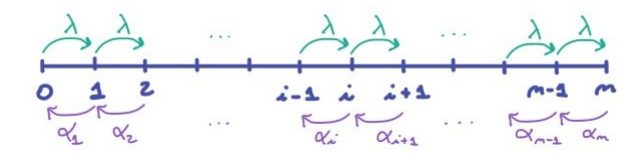
\includegraphics[width=0.75\textwidth]{diagrama_de_las_tasas_de_transicion}
\end{center}
para ciertos valores $\alpha_1, \alpha_2, \dots, \alpha_n$.
\begin{enumerate}
	\item Mostrar que \(\alpha_i = i \mu\) para todo \(1 \leq i \leq n\).
	\item Escribir la matriz de tasas de transición \(Q\) y la matriz de probabilidades de transición asociadas.
	\item Supongamos que \(X_0 = k\) a.s., con \(k \in \{0, 1, \dots, n - 1\}\) (es decir, a tiempo inicial hay \(k\) servidores ocupados).
	\begin{enumerate}[label=\roman*.]
		\item Hallar la probabilidad de que el primer cliente en arribar al sistema encuentre exactamente $k$ servidores ocupados (es decir, que al instante en el que arriba el primer cliente, el proceso $\markovProcess$ pase de $k$ a $k + 1$).
		\item Hallar la probabilidad de que el primer cliente en arribar al sistema encuentre exactamente $i$ servidores ocupados, con $i \in S$.
	(Pensar primero el caso $i = k - 1$, $i = k - 2$, ect.)
		\item Hallar el número esperado de servidores ocupados que encuentra el primer cliente que arriba al sistema.
	\end{enumerate}
\end{enumerate}
\end{exercise}

\begin{proof} 1.
Supongamos que el proceso se encuentra en un estado \(i \in \{1, \dots, n\}\).
Por definición, el proceso saltará al estado \(i - 1\) siguiendo a un reloj \(T \sim \Exp(\alpha_i)\).

Encontrarse en el estado \(i\) equivale a que \(i\) de los \(n\) servidores que forman el sistema se encuentren ocupados atendiendo a un cliente.
Visto de esta manera, el cambio del estado \(i\) al estado \(i - 1\) se dá cuando uno de los \(i\) servidores ocupados finaliza su tarea.
Luego, el cambio del estado \(i\) al estado \(i - 1\) depende de la competencia entre estos servidores.
El tiempo que tarda el \(h\)--ésimo servidor en liberarse es una variable aleatoria \(T_h \sim \Exp(\mu)\);
y el tiempo que transcurre hasta que uno de ellos lo hace es \(\min \{T_1, \dots, T_i\}\).
En particular se sigue \(T = \min \{T_1, \dots, T_i\}\)
Nuestras hipótesis dicen que \(T_1, \dots, T_i\) son mutuamente independientes.
Entonces \(T \sim \Exp(i \mu)\), porque la tasa del mínimo es la suma de las tasas para una familia finita e independiente de distribuciones exponenciales.

La identidad \(\alpha_i  = i \mu\) se sigue de \(T \sim \Exp(\alpha_i)\) y \(T \sim \Exp(i \mu)\).
\end{proof}

% Supongamos que el proceso se encuentra en un estado \(i \in \{1, \dots, n - 1\}\).
% Es decir que de los \(n\) servidores que forman el sistema, \(i\) de ellos se encuentran ocupados atendiendo a un cliente y \(n - i\) estan ociosos.
% Desde este estado, el proceso puede saltar al estado \(i + 1\) o al estado \(i - 1\).
% Saltará al estado \(i + 1\) respondiendo a la llegada de un nuevo cliente.
% Y saltará al estado \(i - 1\) cuando uno de los servidores ocupados finalice su tarea.
% Luego, el cambio partiendo del estado \(i\) depende de la competencia entre \(i + 1\) relojes exponenciales.
% Uno de estos relojes, \(R \sim \Exp(\lambda)\), describe la llegada de nuevos clientes al sistema, y suena a tasa \(\lambda\).
% Los demás \(i\) relojes, \(T_i \sim \Exp(\mu)\) describen los tiempos de duración de las tareas que se encuentran ejecutando los \(i\) servidores activos, y suenan a tasa \(\mu\).
% Por hipótesis todos estos relojes son independientes entre sí.
% Entonces, por las propiedades particulares de las ditribuciones exponenciales, la variable \(\min (T_1, \dots, T_i, R)\) tiene distribución exponencial y su tasa es la suma de las tasas de los relojes \(T_1, \dots, T_i, R\).
% Es decir que el 

%%%%%%%%%%%%%%%%%%%%%%%%%%%%%
\begin{proof}[Cálculo]
Sea \(Q = (q_{i j})_{0 \leq i, j \leq n}\) la matriz generadora del proceso.
Por la definición del proceso mediante el diagrama de las tasas de transición, sabemos que \(Q\) es
\begin{align}
	\begin{pmatrix}
		- \lambda & \lambda \\
		\alpha_1 & -(\lambda + \alpha_1) & \lambda \\
		 & \alpha_2 & -(\lambda + \alpha_2) & \lambda \\
		 & & \ddots & \ddots & \ddots \\
		 & & & \alpha_{n - 2} & -(\lambda + \alpha_{n - 2}) & \lambda \\
		 & & & &\alpha_{n - 1} & -(\lambda + \alpha_{n - 1}) & \lambda \\
		 & & & & &\alpha_n & - \alpha_n
	\end{pmatrix}
\end{align}
Por el ejercicio 2.1., sabemos que \(\alpha_i = i \mu\) para todo \(i \in \{1, 2, \dots, n\}\).
Esto completa la descripción de la matriz \(Q\).

% Nota 7 dic. 2020 Teo de proba práctica clase 23.pdf %
%%%%%%%%%%%%%%%%%%%%%%%%%%%%%%%%%%%%%%%%%%%%%%%%%%%%%%%
% En este documento está la relación entre Q y Pi

Por su parte, la matriz de transición de probabilidad \(\Pi\) de la cadena de Markov asociada al proceso viene dada por \(\pi_{i i} = 0\) para todo \(i \in \{0, 1, \dots, n\}\) porque \(Q \neq 0\), y por \(\pi_{i j} = q_{i j} / Q_i = q_{i j} \left( \sum_{h \in S \setminus j} q_{i h} \right)^{- 1}\) para todo par \(i, j \in \{0, 1, \dots, n\}\) de estados distintos.
Para \(i = 0\), tenemos \(Q_0 = \lambda\).
Para \(i \in \{1, \dots, n - 1\}\), tenemos \(Q_i = i \mu + \lambda\).
Para \(i = n\), tenemos \(Q_n = n \mu\).
Luego \(\Pi\) es
\begin{align}
	\begin{pmatrix}
		 & 1  \\
		\frac{\mu}{\mu + \lambda} & & \frac{\lambda}{ \lambda + \mu} \\ 
		 & \frac{2 \mu}{2 \mu + \lambda} & & \frac{\lambda}{\lambda + 2 \mu} \\
		 & & \frac{3 \mu}{3 \mu + \lambda} & & \frac{\lambda}{\lambda + 3 \mu} \\
		 & & & \ddots & & \ddots \\
		 & & & & \frac{(n - 1) \mu}{(n - 1) \mu + \lambda} & & \frac{\lambda}{\lambda + (n - 1) \mu} \\
		 & & & & & 1
	\end{pmatrix}
\end{align}

\end{proof}





\endgroup

%%%%%%%%%%%%%%%%%%%%%%%%%%%%%%
\begin{exercise}
Sea $(B_t)_{t \geq 0}$ un Movimiento Browniano estándar en dimensión 1.

Para cada $x \in \realnum$ sea $T_x = \inf \{t \geq 0 : B_t = x\}$.
(Notar que \(T_0 = 0\) a.s.)
Denotamos con \(f_{T_x}\) y \(F_{T_x}\) a la función de densidad y a la función de distribución acumuladad de \(T_x\), respectivamente.
\begin{enumerate}[label=\alph*)]
	\item Probar que \(\prob(T_x < + \infty) = 1\) para todo \(x \in \realnum\).
	(Sugerencia: puede ser útil observar el \(\sup_{t \geq 0} B_t\) y el \(\inf_{t \geq 0} B_t\))
	\item Para cada \(x \in \realnum \setminus \{0\}\), calcular \(f_{T_x}\) y verificar que \(\Exp(T_x) = + \infty\).
\end{enumerate}
\end{exercise}

%%%%%%%%%%%%%%%%%%%%%%%%%%%%%%
\begin{exercise}
Sea \((B_t)_{t \geq 0}\) un Movimiento Browniano estándar en dimensión 1, y sean \(x > 0\), \(y > 0\).
Consideremos el stopping time \(T = T_{- y} \wedge T_x\).
\begin{itemize}
	\item Probar que \((B_t^2 - t)_{t \geq 0}\) es una martingala.
	\item Probar que \(\Exp(T) = xy\)
\end{itemize}
\end{exercise}

%%%%%%%%%%%%%%%%%%%%%%%%%%%%%%
\begin{exercise}
(Este ejercicio no es obligatorio)

Sea \((B_t)_{t \geq 0}\) un Movimiento Browniano estándar en dimensión 1, y sean \(a > 0\), y \(b > 0\).
El objetivo es probar que \(\prob(B_t = a + b t \text{ para algún } t > 0) = e^{- 2 a b}\).
\begin{enumerate}[label=\alph*)]
	\item Sea \((X_t)_{t \geq 0}\) el proceso definido por \(X_t = e^{2 b B_t - 2 b^2 t}\).
	Probar que \((X_t)_{t \geq 0}\) es una martingala.
	\item Consideremos el stopping time \(T = \inf \{t > 0 : B_t = a + b t\}\) (donde \(T\) lo definimos como \(\infty\) si ese conjunto es vacío, es decir, si \(B_t < a + b t\) para todo \(t > 0\)).
	Probar que \(\Exp(X_T) \characteristic_{T < \infty} = 1\).
	\item Probar que \(\Exp(X_T \characteristic_{T < \infty}) = e^{2 a b} \prob(T < \infty)\).
	\item Concluir que \(\prob(B_t = a + b t\text{ para algún } t > 0) = e^{- 2 a b}\).
\end{enumerate}
\end{exercise}

\end{document}
